DPC++库由以下组件组成:\par

\begin{itemize}
	\item 经过测试的C++标准API——只需要包含相应的C++标准头文件并使用std命名空间。
	\item 包含相应头文件使用并行STL,只需\#include <dpstd …>,DPC++库就可使用dpstd名称空间。
\end{itemize}

\hspace*{\fill} \par %插入空行
\textbf{DPC++中的标准C++ API}

DPC++库包含一组经过测试的标准C++ API。许多C++标准API的基本功能已经完成,因此这些API可以在设备内核中使用。图18-7展示了如何在设备代码中使用std::swap的示例。\par

\hspace*{\fill} \par %插入空行
图18-7 设备代码中使用std::swap
\begin{lstlisting}[caption={}]
class KernelSwap;
std::array <int,2> arr{8,9};
buffer<int> buf{arr};

{
	host_accessor host_A(buf);
	std::cout << "Before: " << host_A[0] << ", " << host_A[1] << "\n";
} // End scope of host_A so that upcoming kernel can operate on buf

queue Q;
Q.submit([&](handler &h) {
	accessor A{buf, h};
	h.single_task([=]() {
		// Call std::swap!
		std::swap(A[0], A[1]);
	});
});

host_accessor host_B(buf);
std::cout << "After: " << host_B[0] << ", " << host_B[1] << "\n";
\end{lstlisting}

可以使用以下命令来构建和运行程序(假设它位于stdswap.cpp文件中):\par

\begin{tcolorbox}[colback=white,colframe=black]
dpcpp –std=c++17 stdswap.cpp –o stdswap.exe ./stdswap.exe
\end{tcolorbox}

打印结果为:\par

\begin{tcolorbox}[colback=white,colframe=black]
8, 9\\
9, 8
\end{tcolorbox}

图18-8列出了带有“Y”的C++标准API,以表明在编写本文时,这些API已经在用于CPU、GPU和FPGA设备的DPC++内核中进行了测试。空白表示在本书出版时,不完全覆盖(不是所有三种设备类型)。在线DPC++手册中也包含了一个表,并将随着时间的推移而更新——DPC++中的支持将继续扩大。\par

在DPC++库中,一些C++ std函数是基于设备上内置函数的实现,以达到与SYCL版本相同的性能水平。\par

\hspace*{\fill} \par %插入空行
图18-8 库支持CPU/GPU/FPGA覆盖(本书出版时)
\begin{center}
	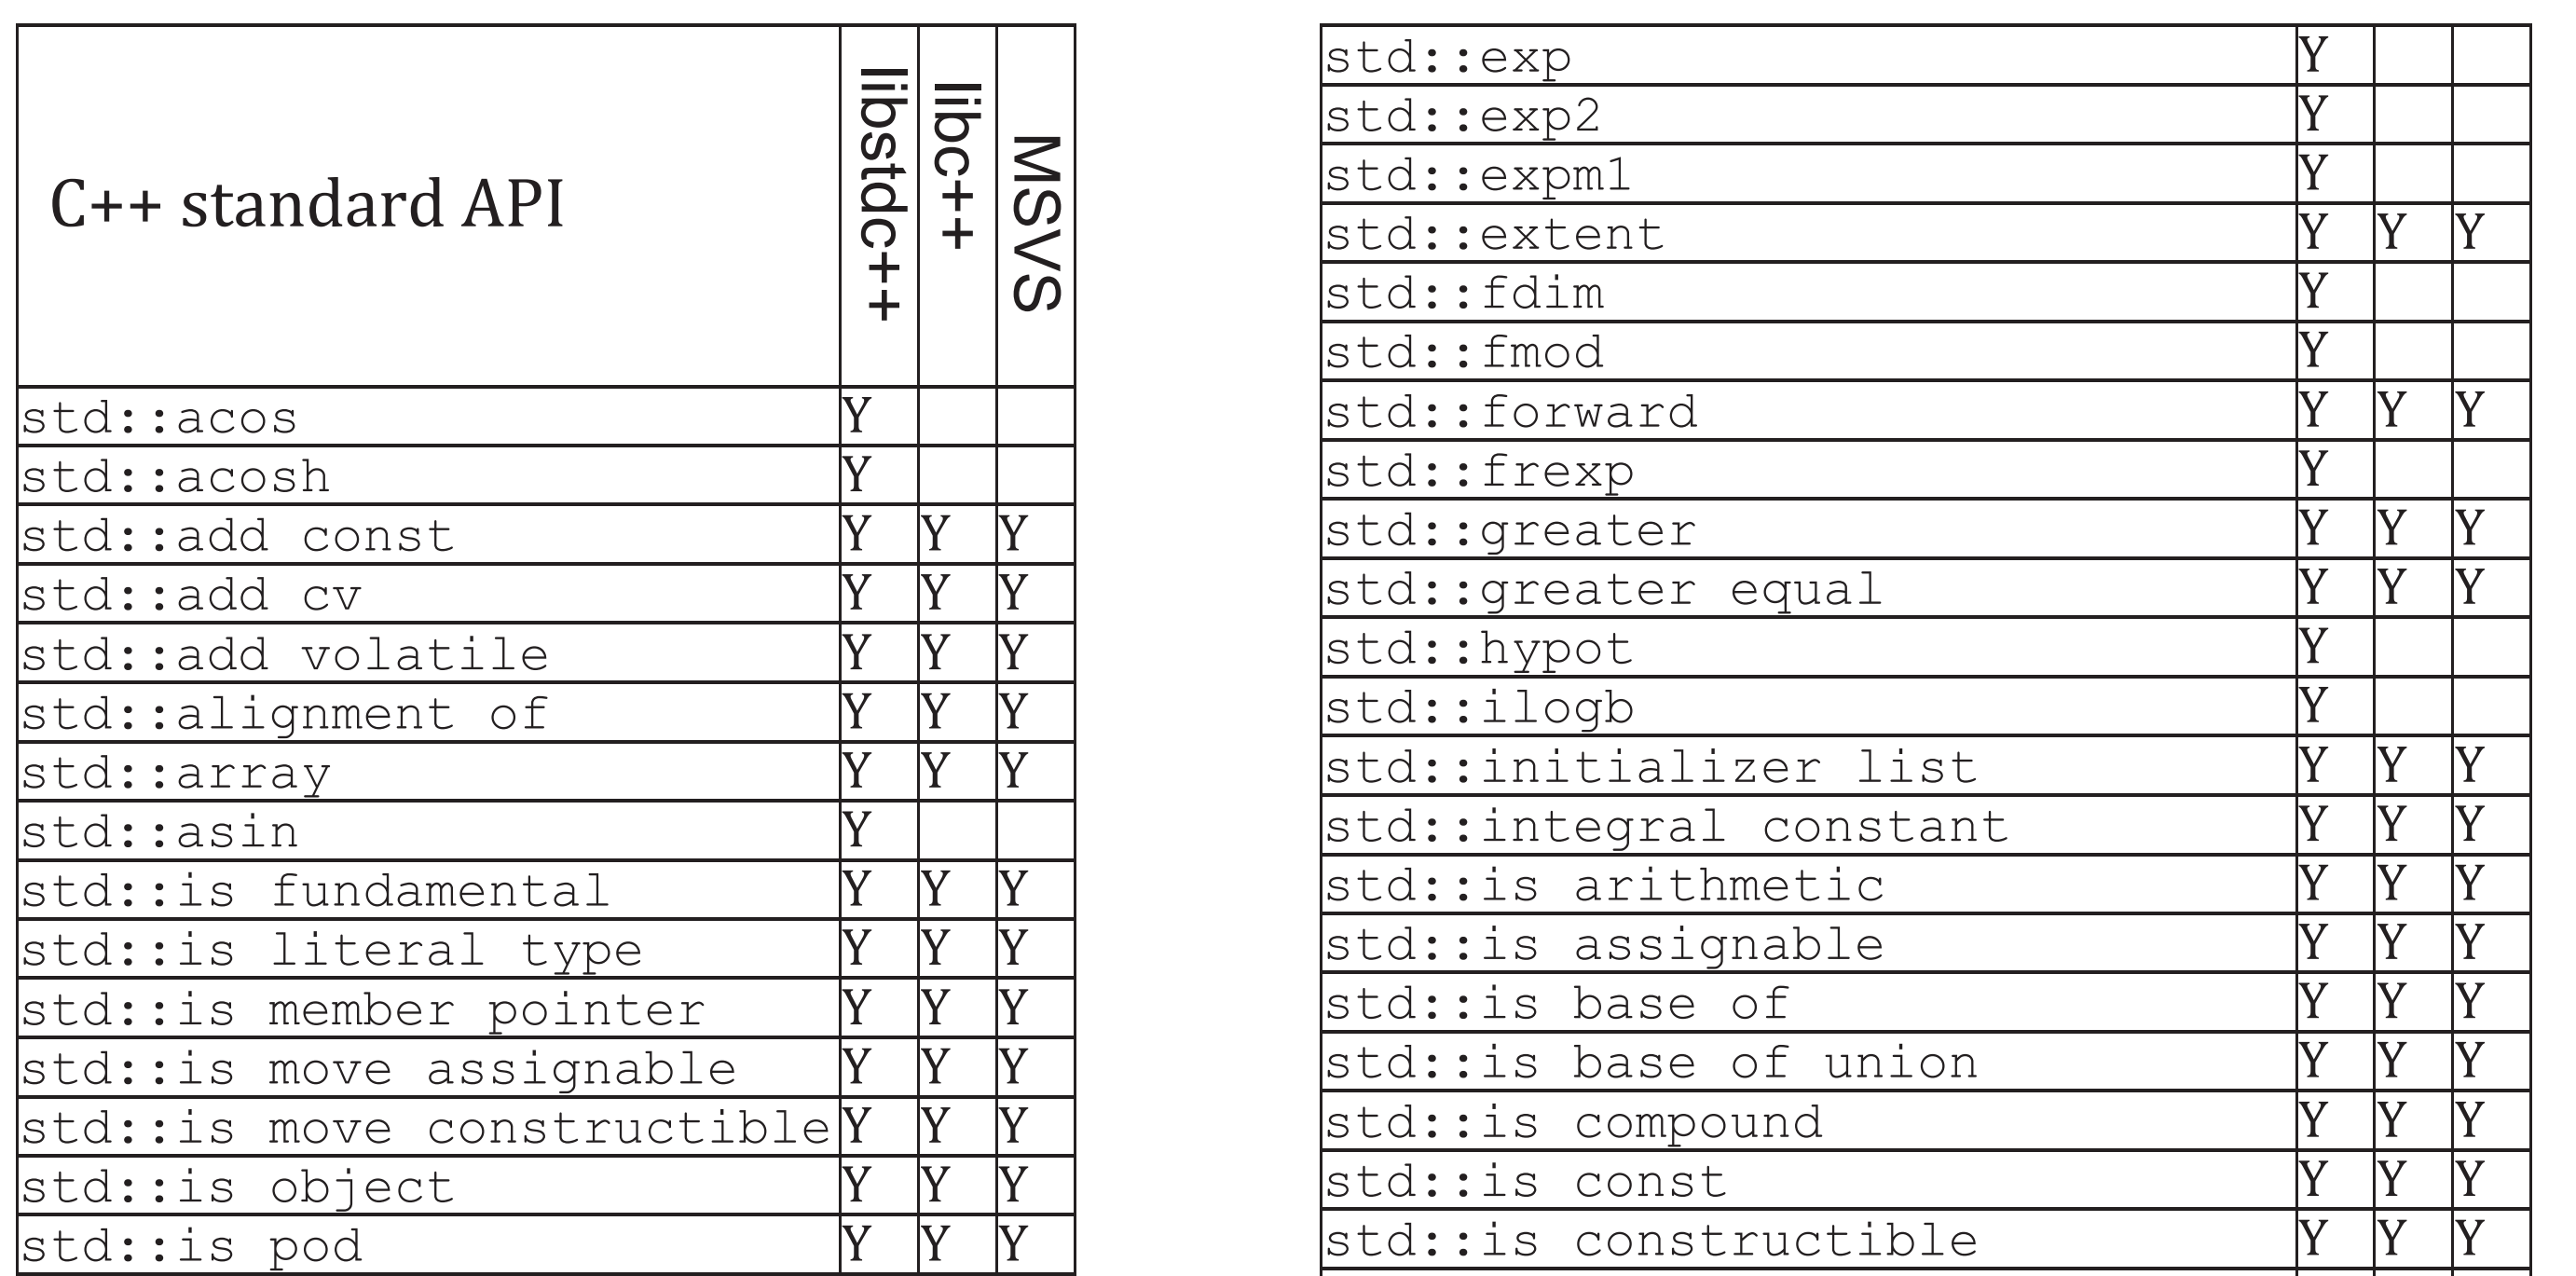
\includegraphics[width=1.0\textwidth]{content/chapter-18/images/7}
	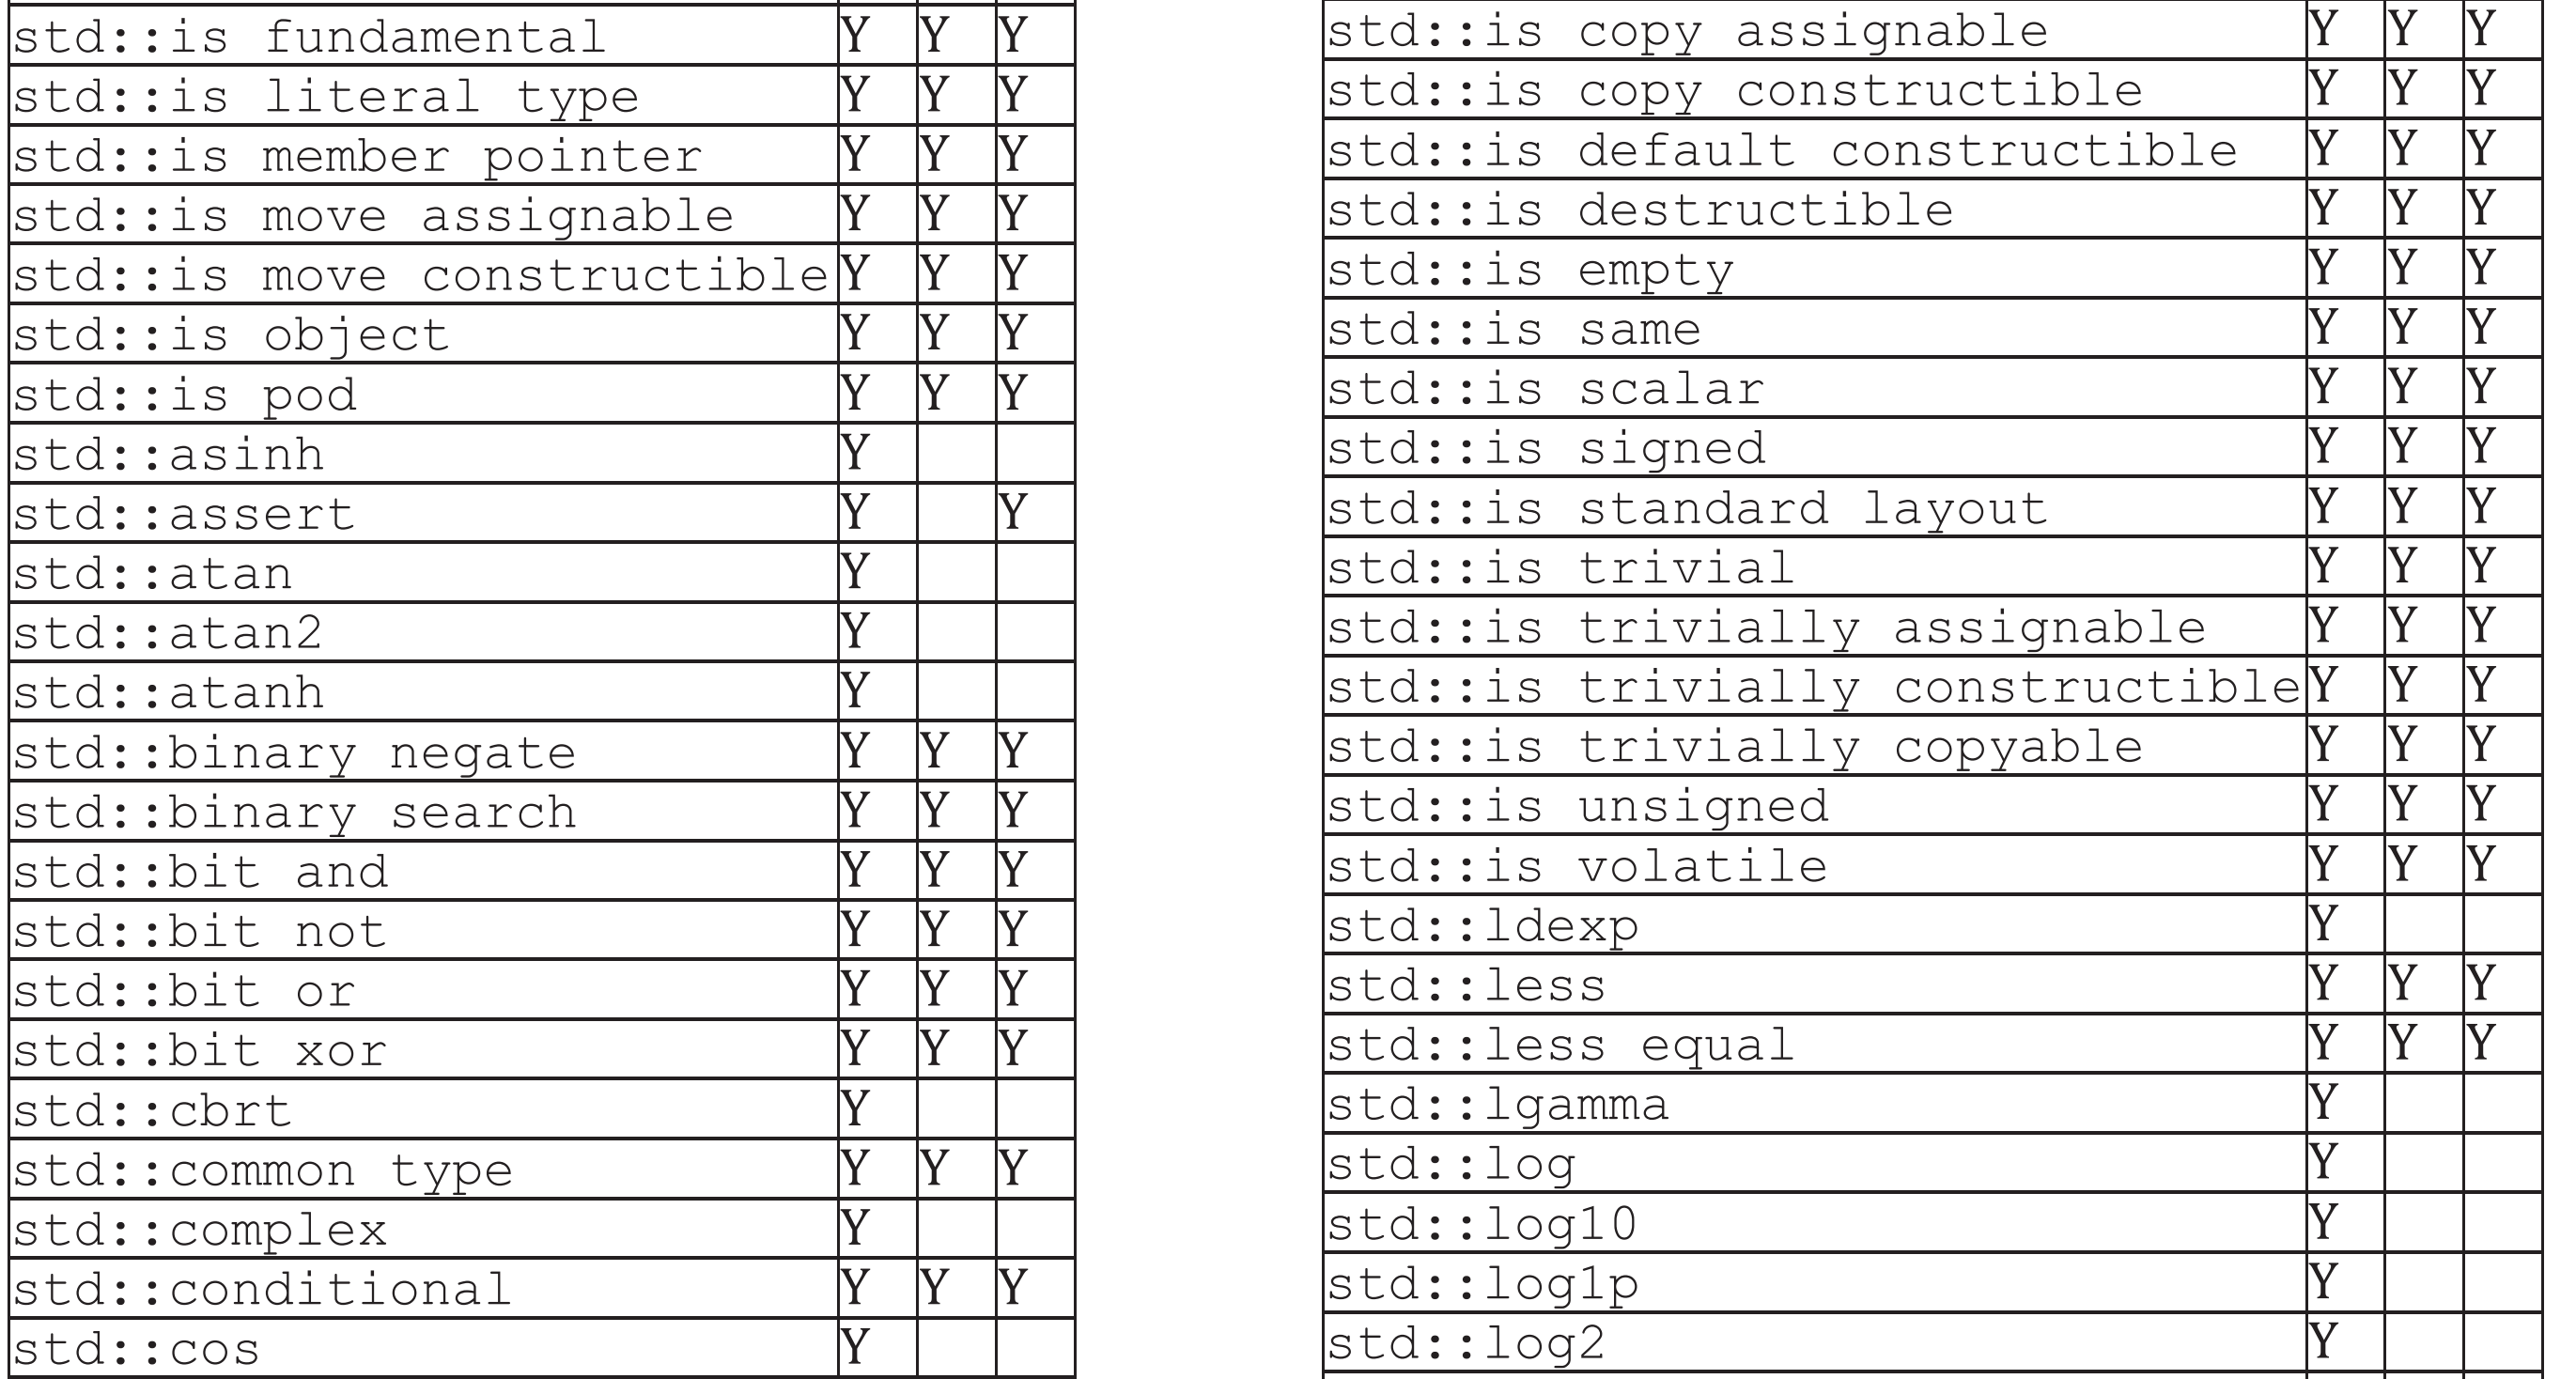
\includegraphics[width=1.0\textwidth]{content/chapter-18/images/8}
	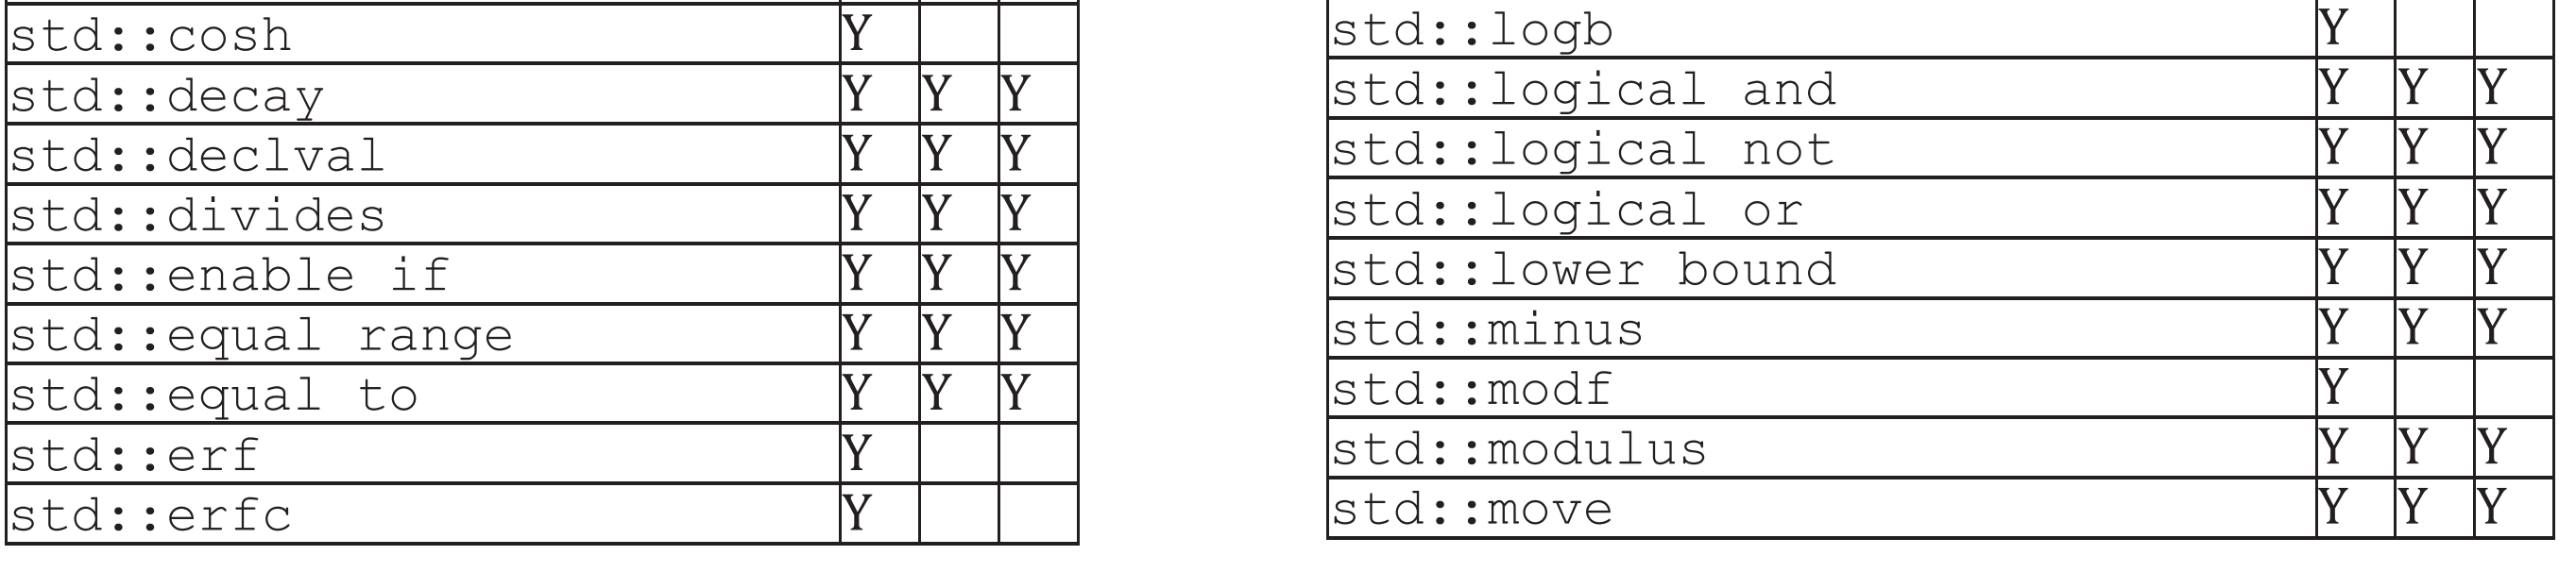
\includegraphics[width=1.0\textwidth]{content/chapter-18/images/9}
	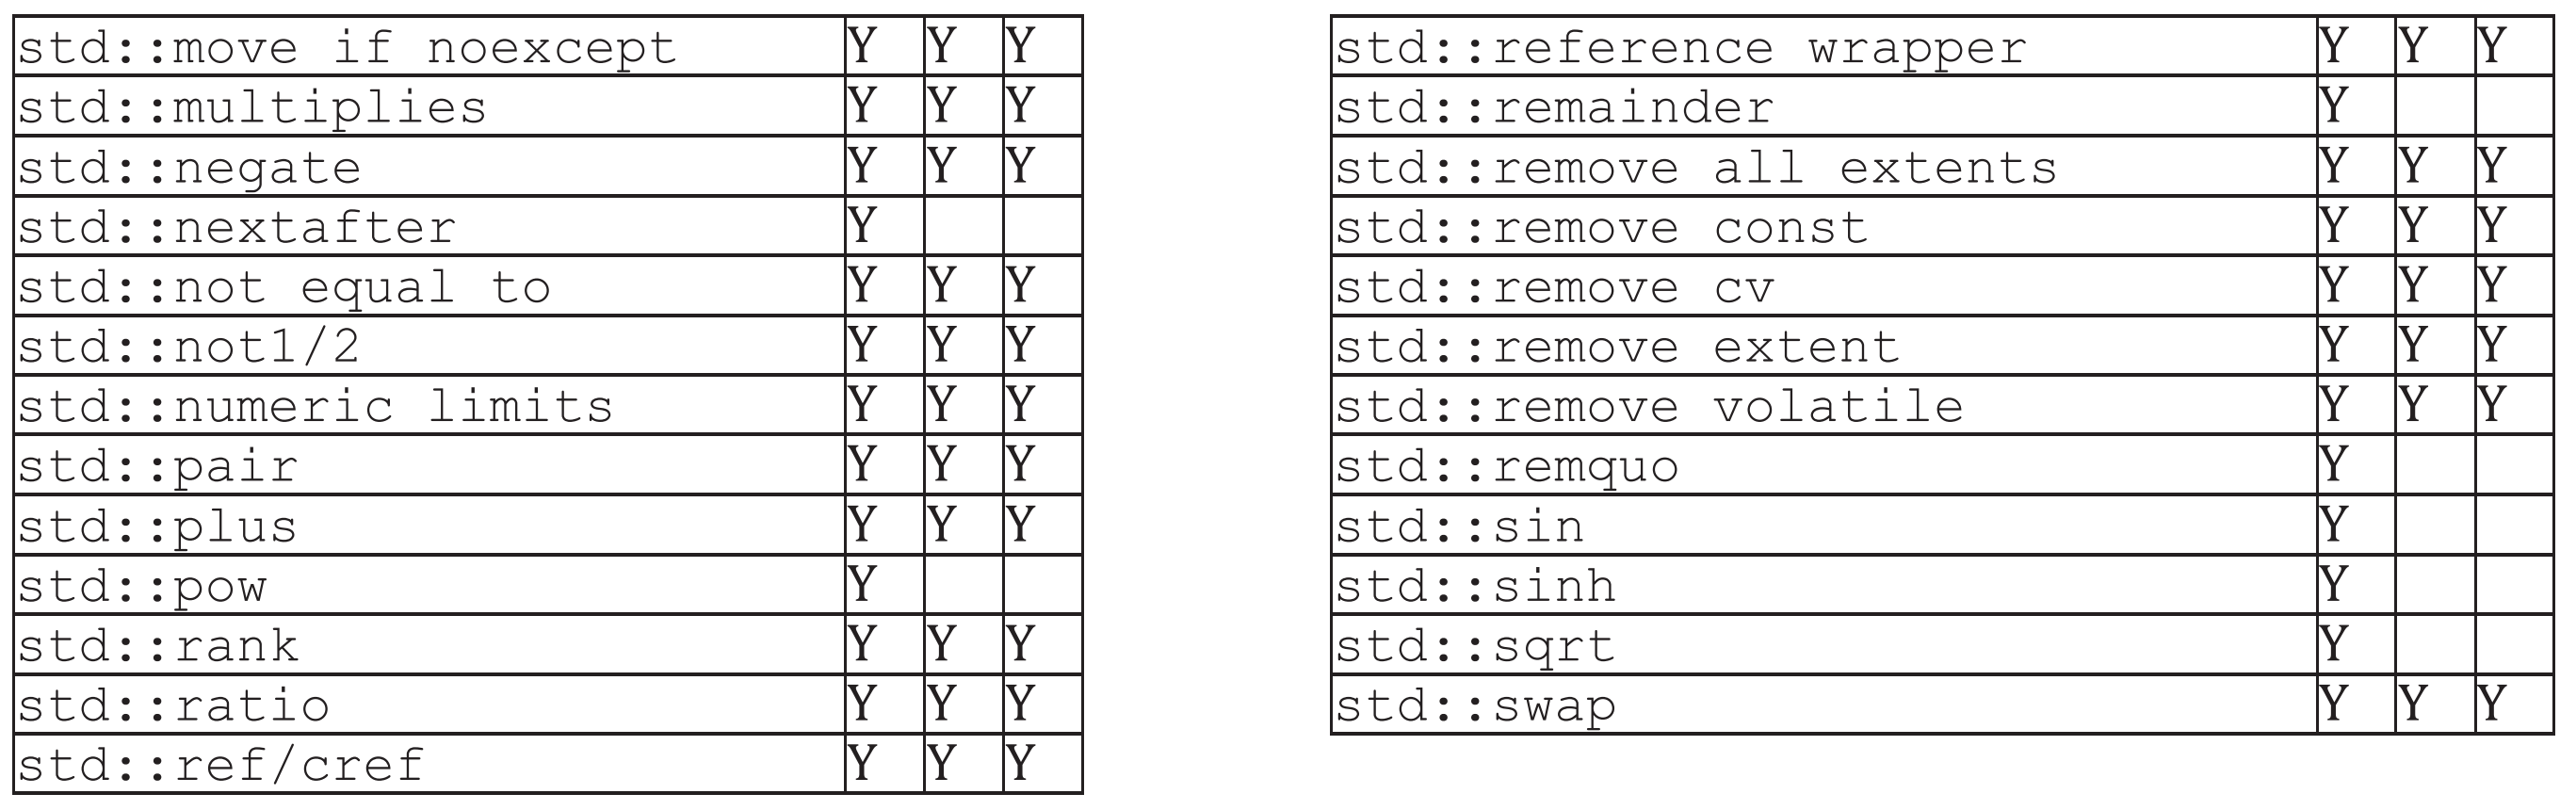
\includegraphics[width=1.0\textwidth]{content/chapter-18/images/10}
\end{center}

在libstdc++ (GNU)与gcc 7.4.0和libc++ (LLVM)与clang 10.0和MSVC标准C++库与Microsoft Visual Studio 2017(主机CPU)支持的标准C++ API。\par

在Linux上,GNU libstdc++是DPC++编译器的默认C++标准库,因此不需要编译或链接选项。如果我们想要使用libc++,请使用编译选项-stdlib=libc++ -nodinc++来使用libc++,不要包含系统中的C++ std头文件。DPC++编译器已经在Linux上的DPC++内核中使用libc++进行了验证,但是DPC++运行时需要用libc++而不是libstdc++重新构建。详情请参见https://intel.github.io/llvmdocs/GetStartedGuide.html\#build-dpc-toolchain-with-libc-library。所以,libc++不是推荐使用的C++标准库。\par

在FreeBSD上,libc++是默认的标准库,-stdlib=libc++选项不是必需的。更多详情请登录https://libcxx.llvm.org/docs/UsingLibcxx.html。在Windows上,只能使用MSVC c++库。\par

\begin{tcolorbox}[colback=red!5!white,colframe=red!75!black]
为了实现跨架构的可移植性,如果std函数在图18-8中没有标记“Y”,在编写设备函数时需要注意是否可移植!
\end{tcolorbox}

\hspace*{\fill} \par %插入空行
\textbf{DPC++的Parallel STL}

Parallel STL是C++标准库算法的实现,支持执行策略,如ISO/IEC 14882:2017标准,通常称为C++17。现有的实现还支持Parallelism TS version 2中指定的未排序执行策略,并在C++工作组P1001R1中为下一版本的C++标准提出了该策略。\par

当使用算法和执行策略时,如果没有特定于C++17的标准库实现,则指定命名空间std::execution,否则指定命名空间pstl::execution。\par

对于任何已实现的算法,都可以将seq、unseq、par或par\_unseq中的值作为调用算法的第一个参数传递,以指定所需的执行策略。这些策略的含义如下:\par

\begin{table}[]
	\begin{tabular}{|l|l|}
		\hline
		执行策略 & 含义                                                                                                                                            \\ \hline
		seq              & 串行执行                                                                                                                              \\ \hline
		unseq            & \begin{tabular}[c]{@{}l@{}}同步执行SIMD。此策略要求在SIMD中安全执行所有函数。\end{tabular} \\ \hline
		par              & 由多个线程并行执行。                                                                                                            \\ \hline
		par\_unseq       & 合并了unseq与par的特性                                                                                                                    \\ \hline
	\end{tabular}
\end{table}

对DPC++的Parallel STL进行了扩展,支持使用特殊执行策略的DPC++设备。DPC++执行策略指定了并行STL算法运行的位置和方式,继承了标准C++的执行策略。封装了一个SYCL设备或队列,并允许设置可选的内核名称。DPC++执行策略可以与所有支持C++17标准执行策略的算法一起使用。\par

\hspace*{\fill} \par %插入空行
\textbf{DPC++执行策略}

目前,DPC++库只支持并行未串行策略(par\_unseq)。使用DPC++执行策略,有三个步骤:\par

\begin{enumerate}
	\item 在代码中添加\#include <dpstd/execution>。
	\item 通过提供标准策略类型、作为模板参数唯一内核名的类型(可选)和以下构造函数参数之一来创建策略对象:
	\begin{itemize}
		\item SYCL队列
		\item SYCL设备
		\item SYCL设备选择器
		\item 具有不同内核名称的已存在策略对象
	\end{itemize}
	\item 将创建的策略对象传递给Parallel STL算法。
\end{enumerate}

dpstd::execution::default\_policy对象是预定义的device\_policy,使用默认的内核名和默认队列创建。这可以用于创建自定义策略对象,或者在调用算法时直接传递(如果默认选择足够的话)。\par

图18-9显示了使用using命名空间dpstd::execution的示例,引用策略类和函数。\par

\hspace*{\fill} \par %插入空行
图18-9 创建执行策略
\begin{lstlisting}[caption={}]
auto policy_b = 
	device_policy<parallel_unsequenced_policy, class PolicyB> 
		{sycl::device{sycl::gpu_selector{}}};
std::for_each(policy_b, …);

auto policy_c = 
	device_policy<parallel_unsequenced_policy, class PolicyС> 
		{sycl::default_selector{}};
std::for_each(policy_c, …);

auto policy_d = make_device_policy<class PolicyD>(default_policy);
std::for_each(policy_d, …);

auto policy_e = make_device_policy<class PolicyE>(sycl::queue{});
std::for_each(policy_e, …);
\end{lstlisting}

\hspace*{\fill} \par %插入空行
\textbf{FPGA的执行策略}

fpga\_device\_policy是一个DPC++策略类,用于在FPGA硬件上实现性能更好的并行算法。在FPGA硬件或FPGA仿真设备上运行应用程序时,可以使用该策略:\par

\begin{enumerate}
	\item FPGA实际设备运行时设置\_PSTL\_FPGA\_DEVICE宏,以及在FPGA仿真器上运行时设置\_PSTL\_FPGA\_EMU宏。
	\item 在代码中添加\#include <dpstd/execution>。
	\item 通过为内核名和展开因子(参见第17章)提供类类型作为模板参数(两个都是可选的)和以下构造函数参数之一来创建策略对象:
	\begin{itemize}
		\item 为FPGA选择器构造的SYCL队列(任何其他设备类型的行为都未定义)
		\item 具有不同内核名称和/或展开因子的FPGA策略对象
	\end{itemize}
	\item 将创建的策略对象传递给Parallel STL算法。
\end{enumerate}

fpga\_device\_policy的默认构造函数创建一个对象,其中包含为FPGA选择器构造的SYCL队列。如果定义了\_PSTL\_FPGA\_EMU,则为FPGA仿真器选择器构造的SYCL队列。\par

dpstd::execution::fpga\_policy是fpga\_device\_policy类的预定义对象,使用默认的内核名称和默认的展开因子创建。使用它来创建定制的策略对象,或者在调用算法时直接使用。\par

图18-10中的代码假设using namespace dpstd::execution;,用于策略,而using namespace sycl;,用于队列和设备选择器。\par

指定策略的展开因子可以在算法的实现中展开循环,默认值为1。了解如何选择更好的值,可以回顾第17章。\par

\hspace*{\fill} \par %插入空行
图18-10 FPGA使用执行策略
\begin{lstlisting}[caption={}]
auto fpga_policy_a = fpga_device_policy<class FPGAPolicyA>{};

auto fpga_policy_b = make_fpga_policy(queue{intel::fpga_selector{}});

constexpr auto unroll_factor = 8;
auto fpga_policy_c = 
make_fpga_policy<class FPGAPolicyC, unroll_factor>(fpga_policy);
\end{lstlisting}

\hspace*{\fill} \par %插入空行
\textbf{使用DPC++ Parallel STL}

为了使用DPC++ Parallel STL,需要通过添加以下行集的子集来包含Parallel STL头文件。头包含哪些文件,取决于所要使用的算法:\par

\begin{itemize}
	\item \#include <dpstd/algorithm>
	\item \#include <dpstd/numeric>
	\item \#include <dpstd/memory>
\end{itemize}

dpstd::begin和dpstd::end是特殊的辅助函数,允许将SYCL缓冲区传递给Parallel STL算法。这些函数接受SYCL缓冲区,并返回一个未指定类型的满足以下要求的对象:\par

\begin{itemize}
	\item 可拷贝构造,可拷贝赋值,并且支持比较操作符==和!=。
	\item 以下表达式是有效的:a+n, a-n, a-b,其中a和b是该类型的对象,n是一个整数值。
	\item 有一个没有参数的get\_buffer,会返回dpstd::begin和dpstd::end的SYCL缓冲区。
\end{itemize}

要使用这些辅助函数,先将\#include <dpstd/iterators>添加到代码中。图18-11和18-12中的代码,使用std::fill函数作为使用开始/结束协助器的示例。\par

\hspace*{\fill} \par %插入空行
图18-11 使用std::fill
\begin{lstlisting}[caption={}]
#include <dpstd/execution>
#include <dpstd/algorithm>
#include <dpstd/iterators>

sycl::queue Q;
sycl::buffer<int> buf { 1000 };

auto buf_begin = dpstd::begin(buf);
auto buf_end = dpstd::end(buf);

auto policy = dpstd::execution::make_device_policy<class fill>( Q );
std::fill(policy, buf_begin, buf_end, 42);
// each element of vec equals to 42
\end{lstlisting}

\begin{tcolorbox}[colback=blue!5!white,colframe=blue!75!black, title=减少主机和设备之间的数据复制]
并行STL算法可以用普通(主机端)迭代器调用,如图18-11中的代码示例所示。\\

本例中,将创建临时SYCL缓冲区,并将数据复制到该缓冲区。设备上的临时缓冲区处理完成后,数据复制回主机。建议直接使用现有的SYCL缓冲区,以减少主机和设备之间的数据移动,以及避免创建和销毁缓冲区的不必要的开销。
\end{tcolorbox}

\hspace*{\fill} \par %插入空行
图18-12 使用默认策略的std::fill
\begin{lstlisting}[caption={}]
#include <dpstd/execution>
#include <dpstd/algorithm>

std::vector<int> v( 1000000 );
std::fill(dpstd::execution::default_policy, v.begin(), v.end(), 42);
// each element of vec equals to 42
\end{lstlisting}

图18-13展示了一个示例,对提供的搜索序列中的每个值执行输入序列的二进制搜索。作为搜索序列的第i个元素的结果,将一个搜索值是否在输入序列中找到的布尔值,赋给结果序列的第i个元素。该算法返回的迭代器指向赋值序列的最后一个元素的下一个位置。该算法假定输入序列已提供了比较排序,如果没有提供比较器,则使用操作符<进行元素比较。\par

前面描述的复杂性强调了应该尽可能利用库函数,而不是自己编写算法实现,这可能需要大量的调试和调优时间。库作者通常都是设备架构的专家,他们可能能看到一些非公开的信息,所以当优化的库可用时,应该先使用。\par

图18-13所示的代码示例演示了使用DPC++并行STL算法时的三个步骤:\par

\begin{itemize}
	\item 创建DPC++的迭代器。
	\item 从现有策略创建命名策略。
	\item 调用并行算法
\end{itemize}

图18-13中的示例使用dpstd::binary\_search算法根据我们的设备选择在CPU、GPU或FPGA上执行二叉搜索。\par

\hspace*{\fill} \par %插入空行
图18-13 使用binary\_search
\begin{lstlisting}[caption={}]
#include <dpstd/execution>
#include <dpstd/algorithm>
#include <dpstd/iterator>

buffer<uint64_t, 1> kB{ range<1>(10) };
buffer<uint64_t, 1> vB{ range<1>(5) };
buffer<uint64_t, 1> rB{ range<1>(5) };

accessor k{kB};
accessor v{vB};

// create dpc++ iterators
auto k_beg = dpstd::begin(kB);
auto k_end = dpstd::end(kB);
auto v_beg = dpstd::begin(vB);
auto v_end = dpstd::end(vB);
auto r_beg = dpstd::begin(rB);

// create named policy from existing one
auto policy = dpstd::execution::make_device_policy<class bSearch>
	(dpstd::execution::default_policy);

// call algorithm
dpstd::binary_search(policy, k_beg, k_end, v_beg, v_end, r_beg);

// check data
accessor r{rB};
if ((r[0] == false) && (r[1] == true) && 
(r[2] == false) && (r[3] == true) && (r[4] == true)) {
	std::cout << "Passed.\nRun on "
	<< policy.queue().get_device().get_info<info::device::name>()
	<< "\n";
} else
	std::cout << "failed: values do not match.\n";
\end{lstlisting}

\hspace*{\fill} \par %插入空行
\textbf{并行STL与USM}

下面的例子描述了并行STL算法与USM结合使用的两种方法:\par

\begin{itemize}
	\item 通过USM指针
	\item 通过USM分配器
\end{itemize}

如果有USM分配器,可以将指向分配开始和结束的指针传递给并行算法。要确保执行策略和分配器本身是为相同的队列或上下文创建的,以避免在运行时出现未定义行为。\par

如果相同的内存要由多个算法处理,可以使用有序队列,或者显式地等待每个算法完成后再在下一个算法中使用相同的内存(这是使用USM时的操作顺序)。也需要等待操作完成后才能访问主机上的数据,如图18-14所示。\par

或者,可以使用std::vector和USM分配器,如图18-15所示。\par

\hspace*{\fill} \par %插入空行
图18-14 使用带有USM指针的并行STL
\begin{lstlisting}[caption={}]
#include <dpstd/execution>
#include <dpstd/algorithm>

sycl::queue q;
const int n = 10;
int* d_head = static_cast<int*>(
	sycl::malloc_device(n * sizeof(int),
						q.get_device(), 
						q.get_context()));
						
std::fill(dpstd::execution::make_device_policy(q),
		  d_head, d_head + n, 78);
q.wait();

sycl::free(d_head, q.get_context());
\end{lstlisting}

\hspace*{\fill} \par %插入空行
图18-15 使用并行STL与USM分配器
\begin{lstlisting}[caption={}]
#include <dpstd/execution>
#include <dpstd/algorithm>

sycl::queue Q;
const int n = 10;
sycl::usm_allocator<int, sycl::usm::alloc::shared> 
						 alloc(Q.get_context(), Q.get_device());
std::vector<int, decltype(alloc)> vec(n, alloc);

std::fill(dpstd::execution::make_device_policy(Q), 
							vec.begin(), vec.end(), 78);
Q.wait();
\end{lstlisting}

\hspace*{\fill} \par %插入空行
\textbf{错误处理与DPC++的执行策略}

如第5章所述,DPC++错误处理模型支持两种类型的错误。对于同步错误,运行时抛出异常,而异步错误只在程序执行期间,会指定用户处理程序错误的时间。\par

对于使用DPC++策略执行的并行STL算法,处理所有错误(同步或异步)是调用者的责任。具体地说\par

\begin{itemize}
	\item 算法不会显式抛出异常。
	\item 运行时在主机CPU上抛出的异常(包括DPC++同步异常),并传递给调用者。
	\item Parallel STL不处理DPC++异步错误,因此必须由程序处理。
\end{itemize}

要处理DPC++异步错误,必须用错误处理程序对象创建与DPC++策略关联的队列。预定义的策略对象(default\_policy和其他)没有错误处理程序,因此如果需要处理异步错误,应该创建自己的策略。\par

































